\documentclass[oneside,intlimits,reqno]{scrbook}

\usepackage{array}
\usepackage{enumerate}
\usepackage{mathrsfs}
\usepackage{mathtools}
\usepackage{pgf,tikz}
\usetikzlibrary{arrows}
\usepackage{extarrows}
\usepackage{graphicx,makeidx}
\usepackage{a4wide}
\usepackage{ragged2e}
\usepackage[nottoc]{tocbibind}
\usepackage{amsmath,amssymb,amsthm,amsfonts}
\usepackage{mathabx}
\usepackage[utf8]{inputenc}
\usepackage[czech]{babel}
\usepackage{relsize}
\usepackage[unicode,breaklinks=true,hypertexnames=false]{hyperref}
\def\dotminus{\mathbin{\ooalign{\hss\raise1ex\hbox{.}\hss\cr
			\mathsurround=0pt$-$}}}

%definice textu nad rovnítkem
\newcommand{\equal}[1]{\mathop{\overset{#1}{\resizebox{\widthof{.{\ensuremath{\mathop{\overset{#1}{\mathop{=}}}}.}}}{\heightof{=}}{$\mathop{=}$}}}}

%redefinice znaků
\renewcommand{\epsilon}{\varepsilon}
\let\crossedphi\phi
\renewcommand{\phi}{\varphi}
\renewcommand{\rho}{\varrho}
\renewcommand{\emptyset}{\font\cmsy = cmsy10 at 12pt\hbox{\cmsy \char 59}}


%definice českých uvozovek
\def\bq{\mbox{\kern.1ex\protect\raisebox{-1.3ex}[0pt][0pt]{''}\kern-.1ex}}
\def\eq{\mbox{\kern-.1ex``\kern.1ex}}
\gdef\uv#1{\bq #1\eq}


\renewcommand{\d}{\mathrm{d}} % diferenciál
\newcommand{\me}{\mathrm{e}} % eulerovo číslo
\newcommand{\E}{\mathbb{E}} % střední hodnota
\newcommand{\D}{\mathrm{D}} %  rozptyl
\newcommand{\LL}{\mathscr{L}}
\newcommand{\Loss}{\mathscr{L}}
\newcommand{\FF}{\mathrm{F}} % distribuční funkce
\newcommand{\PP}{\mathbb{P}} % pravděpodobnost
\newcommand{\NN}{\mathcal{N}}
\newcommand{\MSE}{\mathrm{MSE}}
\newcommand{\LSE}{\mathrm{LSE}}
\newcommand{\Exp}{\mathrm{Exp}}
\newcommand{\NF}{\mathrm{F}}
\newcommand{\AN}{\mathcal{AN}}
\newcommand{\sgn}{\mathrm{sgn}}
\newcommand{\A}{\mathrm{A}}

\newcommand{\prostor}{(\Omega,\mathcal{A},\PP)} % prostor
\newcommand{\mi}{\mathrm{i}} % imaginární jednotka
\newcommand{\R}{\mathbb{R}} % množina reálných čísel
\renewcommand{\C}{\mathbb{C}} % množina komplexních čísel
\newcommand{\Z}{\mathbb{Z}} % množina celých čísel
\newcommand{\N}{\mathbb{N}} % množina přirozených čísel
\newcommand{\Cc}{\mathcal{C}} % funkce třídy C (spojité)
\newcommand{\I}{\mathbb{I}} % identita
\newcommand{\Identita}[1]{\mathbb{I}_{#1}} % identita
\newcommand{\fisher}{\mathbb{I}} % Fisherova matice
\newcommand{\RR}{\mathcal{R}}
\newcommand{\Be}{\mathrm{Be}}
\newcommand{\Bi}{\mathrm{Bi}}
\newcommand{\X}{\textbf{X}}
\newcommand{\Y}{\textbf{Y}}

\newcommand{\PEX}{\PP^\X}
\newcommand{\fex}{f_\X}
\newcommand{\FEX}{\FF_\X}


\newcommand{\Aa}{\mathcal{A}}
\newcommand{\Bb}{\mathcal{B}}
\renewcommand{\t}{\theta} % theta
\newcommand{\bmu}{\boldsymbol{\mu}} % vektorové mí

\newcommand{\htm}{\widehat{\t}_\txt{M}}
\newcommand{\html}{\widehat{\t}_\txt{ML}}
\newcommand{\htn}{\widehat{\t}_n}
\newcommand{\rhn}{R_{H_0}}
\newcommand{\Phiast}{\crossedphi^\ast}
\newcommand{\rhno}{\overline{R}_{H_0}}
\newcommand{\freg}{\mathcal{F}_{reg}}
\newcommand{\fregp}{\mathcal{F}_{reg}^+}
\newcommand{\fregml}{\mathcal{F}_{reg}^\txt{ML}}
\newcommand{\RE}{\mathrm{RE}_{2,1}}
\newcommand{\ARE}{\mathrm{ARE}_{2,1}}


%matematické výrazy
\newcommand{\tg}{\mathop{\mathrm{tg}}}
\newcommand{\argmin}{\mathop{\mathrm{argmin}}}
\newcommand{\argmax}{\mathop{\mathrm{argmax}}}
\newcommand{\argsup}{\mathop{\mathrm{argsup}}}
\renewcommand{\Re}{\mathop{\mathrm{Re}}}
\newcommand{\Ran}{\mathop{\mathrm{Ran}}}
\newcommand{\supp}{\mathop{\mathrm{supp}}}
\renewcommand{\Im}{\mathop{\mathrm{Im}}}
\newcommand{\Cov}{\mathbb{C}\mathrm{ov}}


%konvergence
\newcommand{\sj}{\stackrel{s.j.}{\longrightarrow}}
\newcommand{\Pto}{\stackrel{\PP}{\to}}
\newcommand{\wto}{\stackrel{w}{\to}}
\newcommand{\Dto}{\stackrel{\mathscr{D}}{\to}}
\newcommand{\PSJ}{\stackrel{\PP,s.j.}{\longrightarrow}}
\newcommand{\Lto}{\stackrel{(\mathscr{L})}{\to}}
\newcommand{\sjP}{\stackrel{s.j.~\PP}{\longrightarrow}}
\newcommand{\Lp}{\stackrel{L_p}{\longrightarrow}}

%nadtržítka
\newcommand{\overbar}[1]{\mkern 1mu\overline{\mkern-1mu#1\mkern-3mu}\mkern 3mu}
\newcommand{\Oxn}{\overbar{\rule{0ex}{1.8ex}X_n}}
\newcommand{\Oyn}{\overbar{\rule{0ex}{1.8ex}Y_n}}
\newcommand{\Ox}[1]{\overbar{\rule{0ex}{1.8ex}X_{#1}}}
\newcommand{\Oy}[1]{\overbar{\rule{0ex}{1.8ex}Y_{#1}}}
\newcommand{\oxn}{\overbar{\rule{0ex}{1.33ex}X_n}}
\newcommand{\ox}[1]{\overbar{\rule{0ex}{1.33ex}X_{#1}}}
\newcommand{\oy}[1]{\overbar{\rule{0ex}{1.33ex}Y_{#1}}}
\newcommand{\oyn}{\overbar{\rule{0ex}{1.33ex}Y_n}}
\newcommand{\omn}{\overbar{\rule{0ex}{1.3ex}\mu_n}}

\newcommand{\oxnn}{\overbar{\rule{0ex}{1.33ex}x_n}}
\newcommand{\oynn}{\overbar{\rule{0ex}{1.33ex}y_n}}

%stříšky
\newcommand{\hsn}{\widehat{\sigma}_n^2}

%posloupnosti
\newcommand{\posl}{(X_j)_{j=1}^{+\infty}}
\newcommand{\poslkon}{(X_j)_{j=1}^{n}}
\newcommand{\posln}{(X_n)_{n=1}^{+\infty}}
\newcommand{\poslnn}{(\X_n)_{n=1}^{+\infty}}

%sumy
\newcommand{\suminftyo}{\sum\limits_{n=0}^{+\infty}}
\newcommand{\suminfty}{\sum\limits_{n=1}^{+\infty}}
\newcommand{\sumainfty}[1]{\sum\limits_{#1}^{+\infty}}
\newcommand{\suminftylo}{\sum\limits_{l=0}^{+\infty}}
\newcommand{\sumjn}{\sum\limits_{j=1}^{n}}
\newcommand{\sumin}{\sum\limits_{i=1}^{n}}
\newcommand{\sm}[2]{\sum\limits_{ #1 }^{ #2 }}


\newcommand{\dom}[1]{\mathop{\mathrm{Dom} (#1)}} % definiční obor
\newcommand{\mat}[1]{\mathbf #1}
\newcommand{\abs}[1]{\left|#1\right|}
\renewcommand{\b}[1]{\left( #1 \right)}
\newcommand{\nor}[1]{\left\|#1\right\|}
\newcommand{\Br}[1]{\Bigl(#1\Bigr)}
\newcommand{\br}[1]{\bigl(#1\bigr)}
\newcommand{\e}[1]{\me^{#1}}
\newcommand{\inv}[1]{#1^{-1}}
\newcommand{\ini}{\theta\in\Theta}
\newcommand{\init}[1]{\theta\in\Theta\subset\R^#1}
\newcommand{\txt}[1]{\mathrm{{\footnotesize  #1 }}}
\newcommand{\matice}[4]{\left(\begin{array}{cc}	#1 & #2 \\ #3 & #4	\end{array} \right)}
\newcommand{\maticehrana}[4]{\left[\begin{array}{cc}	#1 & #2 \\ #3 & #4	\end{array} \right]}
\newcommand{\vektor}[2]{\left(\begin{array}{c}	#1  \\  #2	\end{array} \right)}
\newcommand{\p}[1]{\PP\left( #1 \right)}
\newcommand{\EE}[1]{\E\left[ #1 \right]}
\newcommand{\n}[1]{\NN\left( #1 \right)}
\newcommand{\hypothesis}[2]{H_0: #1 ~\text{vs.}~ H_1: #2 }
\newcommand{\hypothesiswide}[2]{H_0: #1 \qquad\text{vs.}\qquad H_1: #2 }
\newcommand{\silofunkce}[1]{\beta_\crossedphi\big|_{\Theta_{#1}}}
\newcommand{\silofunkceast}[1]{\beta_{\Phiast}\big|_{\Theta_{#1}}}
\newcommand{\hypothesisap}[2]{H'_0: #1 ~\text{vs.}~H'_1: #2 }
\newcommand{\test}[1]{\boxed{\text{TEST: $H_0$ zamítáme, pokud } #1 .}}
\renewcommand{\S}{\mathbb{S}}


% Prostředí
\theoremstyle{definition}
\newtheorem{define}{Definice}[chapter]
\theoremstyle{plain}
\newtheorem{theorem}[define]{Věta}
\newtheorem{lemma}[define]{Lemma}
\newtheorem{dusl}[define]{Důsledek}
\newtheorem{corollary}[define]{Tvrzení}
\renewcommand{\proofname}{Důkaz}

\theoremstyle{remark}
\newtheorem{example}[define]{\textsc{Příklad}}
\newtheorem{remark}[define]{\textsc{Poznámka}}

\renewcommand{\indexname}{Rejstřík}

\frenchspacing

\begin{document}
\section{Jednorozměrná lineární regrese}

předpokládejme, že sledujeme dvě veličiny $ x $ a $ y $ mezi kterými existuje lineární závislost

\begin{equation}
	y = \beta_{0} + \beta_{1} x   \quad \text{kde} \quad \beta_{0}, \beta_{1} \quad \text{neznáme.} 
\end{equation}

Provede se experiment a zjistí se hodnoty dvojic ($ x , y $). Často se stává, že $ x $ je změřeno prakticky zcela přesně.

\begin{remark}
 To nastává například v případě, kdy se $ x $ nastavuje na předem dané úrovni a následně se k němu změří odpovídající $ y $.
\end{remark}
 
Oproti tomu u $ y $ obvykle předpokládáme měření s chybou. Chyba může být náhodná a proto i $ y $ budeme chápat jako náhodnou veličinu, kterou budeme značit $ Y $. Pro dvojice $ (x_{1}, Y_{1}), \dots ,( x_{n}, Y_{n} )$ se zavádí model

\begin{equation}\label{eq:lin_reg_model}
	Y_{i} = \beta_{0} + \beta_{1} x_{i} + e_{i} \quad \text{kde} \quad i = 1, \dots ,n .
\end{equation}

Jednotlivé proměnné se pak nazývají následovně

\begin{itemize}
  \item $ Y_{i} $ -- vysvětlovaná (závislá) proměnná
  \item $ x_{i} $ -- vysvětlující (nezávislá) proměnná, \textit{popřípadě prediktor nebo regresor}
  \item $ \beta_{0},\beta_{1} $ -- neznámé regresní parametry
  \item $ e_{i} $ -- náhodný šum, (náhodná chyba)
\end{itemize}

Budeme předpokládat, že $ e_{i} $ jsou nezávislé (někdy bude dokonce stačit, aby byly nekorelované) a $ e_{i} \sim (0,\sigma ^{2}) $. A tedy splňuje $ \mathbb{E} [ e_{i} ]  = 0 $ , $ \textbf{Var} [ e_{i} ] = \sigma ^{2} $ pro $ \forall i $ (homoskedasticita).

Měřením získáme data $ (x_{1}, y_{1}), \dots ,( x_{n}, y_{n} )$ a cílem statistické analýzy je určit, zda model\,(\eqref{eq:lin_reg_model}) schopen popsat pozorovanou variabilitu u $ y $. 

\textbf{První krok }

Odhadneme neznámé parametry $ \beta_{0}, \beta_{1}, \sigma^{2} $. Proložíme data přímkou ve tvaru
\begin{equation}\label{eq:lin_reg_model}
	\widehat{y}(x) = \widehat{\beta}_{0} + \widehat{\beta}_{1} x 
\end{equation}
a porovnáme $ y_{i} $ -- \textit{naměřená data} a $ \widehat{y}(x_{i}) $ -- \textit{predikovaná hodnota lineární regrese} pro $ \forall i $. To nám umožňuje posoudit adekvátnost modelu.

Pro proložení dat přímkou existuje několik způsobů. Zásadní ovšem bude znalost rozdělení $ e_{i} $ a tady i $ Y_{i} $ i když apriori není zřejmé proč znát rozdělení a ne $ \beta_{0}, \beta_{1} $.

Zde máme následující možnosti:

\begin{enumerate}
  \item Odhadnout $ \beta_{0} , \beta_{1} $ pomocí metody nezávisející na rozdělení chyb
  \item Udělat věrohodnostní předpoklad o rozdělení chyb, odhadnout $ \beta_{0} , \beta_{1} $ a následně ověřit předpoklad
\end{enumerate}


\begin{remark}
 Speciální důležitý případ je $ e_{i} \sim \text{N}(0,\sigma^{2}) $ který při MLE odhadu $ \beta_{0}, \beta_{1} $ vede na metodu nejmenších čtverců, která může být použita bez ohledu na rozdělení chyb.
\end{remark}

\textbf{Odhady parametrů}
\subsection{Předpoklad normality dat}
Předpokládáme, že $ e_{1}, \dots , e_{n} $ i.i.d. $ \text{N}(0,\sigma^{2}) $. To znamená, že $ Y_{i} \sim \text{N}(\beta_{0} + \beta_{1} x_{i},\sigma^{2}) $ a jednotlivé $ Y_{1}, \dots , Y_{n} $ jsou nezávislé.

\textbf{MLE odhady}

Věrohodnostní funkce je ve tvaru

\begin{equation}
\begin{aligned}
	L = L ( \beta_{0} , \beta_{1} , \sigma^{2} ) = \left( \frac{1}{ \sqrt{ 2 \pi \sigma^{2} }} \right) ^{n} \text{exp} \left( - \dfrac{1}{2 \sigma^{2} } \sum_{i = 1}^{n}( y_{i} -  \beta_{0}  - \beta_{1} x_{i} )^{2} \right) \\
l = \text{ln} L = -\frac{n}{2} \text{ln} ( 2 \pi ) -\frac{n}{2} \text{ln} (\sigma^{2} ) - \dfrac{1}{2 \sigma^{2} } \sum_{i = 1}^{n}( y_{i} -  \beta_{0}  - \beta_{1} x_{i})^{2}
\end{aligned}
\end{equation}

pro pevné $ \sigma^{2} > 0 $ je maximalizace $ l $ ekvivalentní s minimalizováním $ S $, kde

\begin{equation}
S = S ( \beta_{0} , \beta_{1} ) = \sum_{i = 1}^{n}( y_{i} -  \beta_{0}  - \beta_{1} x_{i})^{2}.
\end{equation}

Proto tuto metodu někdy nazýváme metodou nejmenších čtverců.

\begin{equation}
\begin{aligned}
\dfrac{\partial S}{\partial \beta_{0}} = - 2 \sum_{i = 1}^{n}( y_{i} -  \beta_{0}  - \beta_{1} x_{i}) = 0 , \\
\dfrac{\partial S}{\partial \beta_{1}} = - 2 \sum_{i = 1}^{n}( y_{i} -  \beta_{0}  - \beta_{1} x_{i}) x_{i}= 0 .
\end{aligned}
\end{equation}
Z první rovnice pak dostaneme
\begin{equation}
 \beta_{0} = \dfrac{1}{n} \sum_{i = 1}^{n} y_{i} -  \beta_{1}  - \dfrac{1}{n} \sum_{i = 1}^{n} x_{i} = \overline{y}_{n} - \beta_{1} \overline{x}_{n}
\end{equation}
a dosazením do druhé dostaneme výraz
\begin{equation}
\begin{aligned}
\sum_{i=1}^{n} y_{i} x_{i} - \beta_{0} \sum_{i=1}^{n} x_{i} - \beta_{1} \sum_{i=1}^{n} x_{i}^{2} = 0 , \\
\sum_{i=1}^{n} y_{i} x_{i} - \overline{y}_{n} \sum_{i=1}^{n} x_{i} - \beta_{1} \overline{x}_{n} \sum_{i=1}^{n} x_{i} - \beta_{1} \sum_{i=1}^{n} x_{i}^{2} = 0. \\
\end{aligned}
\end{equation}
Jednotlivé MLE odhady parametrů pak mají následující tvar
\begin{equation}
\widehat{\beta}_{0} = \overline{y}_{n} - \widehat{\beta}_{1} \overline{x}_{n} \quad a \quad
\widehat{\beta}_{1} = \dfrac{\sum_{i=1}^{n} y_{i} x_{i} - n \overline{x}_{n} \overline{y}_{n}}{\sum_{i=1}^{n} x_{i}^{2} - n \overline{x}_{n}^{2}}.
\end{equation}

Nyní najdeme odhad parametru $ \sigma^{2} $ 

\begin{equation}
\frac{ \partial l}{ \partial \sigma^{2}} = -\frac{n}{2} \cdot \dfrac{1}{\sigma^{2}} + \dfrac{1}{2 (\sigma^{2})^{2}} \sum_{i=1}^{n} ( y_{i} -  \beta_{0}  - \beta_{1} x_{i})^{2} = 0,
\end{equation}
vyjádřením $ \sigma^{2} $ z rovnice dostaneme výraz
\begin{equation}
\widehat{\sigma}^{2} = \frac{1}{n} \sum_{i=1}^{n} ( y_{i} -  \beta_{0}  - \beta_{1} x_{i})^{2} = \frac{1}{n} \sum_{i=1}^{n} ( y_{i} -  \widehat{y}_{i})^{2} = \dfrac{1}{n} \text{SSE},
\end{equation}
kde $ \widehat{y}_{i} = \beta_{0}  - \beta_{1} x_{i} $ je predikce modelu (odhad $ \mathbb{E} [ Y_{i} ] $ ) a  zkratka SSE je odvozena z anglického \textit{sum of the squares of errors}. Rozdíl $ \widehat{e}_{i} = y_{i} -  \widehat{y}_{i} $ nazýváme $ i $--té reziduum. Velikost reziduí indikuje, jak dobře odhadnutá přímka odpovídá datům. Rezidua jsou vlastně odhady chyb $ e_{i} $,  jejich analýza hraje významnou roli v ověření předpokladů rozdělení chyb.

\begin{remark}
Pro odhad $ \sigma^{2} $ se používá častěji statistika $ s^{2}_{n} = \dfrac{1}{n - 2} \sum_{i=1}^{n}(y_{i} -  \widehat{y}_{i})^{2} = \dfrac{1}{n-2} \text{SSE} $, která je nestranným odhadem parametru $ \sigma^{2} $ (pro libovolné rozdělení $ e_{i} $), zatímco $ \sigma^{2}_{\text{MLE}} $ je vychýlený odhad i pro normální rozdělení chyb.
\end{remark}
\textbf{Odhad $ \sigma $}

pro odhad parametru $ \sigma $ využíváme statistiku nazývanou standardní chyba regrese (standard error), která má tvar
\begin{equation}
 s_{n} = \sqrt{\dfrac{1}{n-2} \sum_{i=1}^{n}(y_{i} -  \widehat{y}_{i})^{2}}.
\end{equation}
Tento odhad není nestranný.

\subsection{Data bez předpokladu normality}
Bez předpokladu normality chyb. Tedy, že $ e_{1}, \dots , e_{n} $ jsou nekorelované, $ e_{1}, \dots , e_{n} \sim (0,\sigma^{2}) $.
Pro odhad $ \beta_{0}, \beta_{1} $ lze použít minimalizaci S (nejmenší čtverce), což je rozumné provedení, když si uvědomíme ?????? interpret??? (strana 5).

Nechť $ y = \beta_{0} + \beta_{1} x  $ je rovnice nějaké přímky, potom $ y_{i} - (\beta_{0} + \beta_{1} x_{i}) $ je vertikální vzdálenost bodu $ (x_{i},y_{i}) $ od přímky a 
\begin{equation}
 S = \sum_{i=1}^{n} (y_{i} - \beta_{0} - \beta_{1} x_{i})^{2}
\end{equation}
je míra udávající, jak dobře přímka prokládá data. Dává smysl vybrat takovou přímku, která minimalizuje S. Minimalizací S získáme stejné odhady $  \widehat{\beta}_{0}, \widehat{\beta}_{1} $ jako u MLE odhadů pro normální data. Teď se ale nazývají odhad metodou nejmenších čtverců LSE (least squares estimators).
Existuje více měr vhodnosti přímky. Použití LSE pro libovolné rozdělení chyb má dvě zdůvodnění.
\begin{enumerate}
  \item pro normální rozdělení chyby LSE splývá s MLE.
  \item LSE odhad je navíc BLUE (best linear unbiased estimator) jak ukážeme v Gauss–Markov theorem
\end{enumerate}

\begin{example}
Nechť $ e_{1}, \dots , e_{n} $ jsou i.i.d. s hustotou
\begin{equation*}
  f(\epsilon) = \dfrac{1}{2} e ^{- \vert \epsilon \vert} \quad \text{Laplaceovo rozdělení}
\end{equation*}
potom hustota $ Y_{i} $ je 
\begin{equation*}
  f_{Y_{i}}(y_{i}) = \dfrac{1}{2} e ^{- \vert y_{i} - \beta_{0} - \beta_{1} x_{i} \vert} 
\end{equation*}
a věrohodnostní funkce $ L $ a $  l$ mají tvar
\begin{equation*}
\begin{aligned}
  L = \dfrac{1}{2^{n}} e ^{- \sum_{i=1}^{n} \vert y_{i} - \beta_{0} - \beta_{1} x_{i} \vert}  \\
  l = -n \text{ln} 2 - \sum_{i=1}^{n} \vert y_{i} - \beta_{0} - \beta_{1} x_{i} \vert 
\end{aligned} 
\end{equation*}
MLE odhady parametrů $ \beta_{0} , \beta_{1} $ získáme minimalizací
\begin{equation}
A = \sum_{i=1}^{n} \vert y_{i} - \beta_{0} - \beta_{1} x_{i} \vert \quad \dots \text{ \, MAD (minimum absolute deviation).}
\end{equation}
Zde budou odhady jiné než u LSE.

Uvažujme 3 body: $ (0,0) , (1,0) , (\dfrac{1}{2},\dfrac{1}{2}) $.
\begin{equation}
\begin{aligned}
\text{MLE: } \quad  \beta_{0} = \beta_{1} = 0 \quad , \quad A = 0.5
 \quad , \quad \widehat{y} = 0 \\
 \text{LSE: } \quad \overline{x} = \dfrac{1}{2} \, , \, \overline{y} = \dfrac{1}{6} \quad , \quad \sum_{i=1}^{n} x_{i}^{2} = \dfrac{5}{4} \, , \, \sum_{i=1}^{n} x_{i} y_{i} = \dfrac{1}{4} \quad , \quad \beta_{1} = 0 \, , \, \beta_{0} = \dfrac{1}{6}
  \end{aligned}  
\end{equation}
\begin{center}
    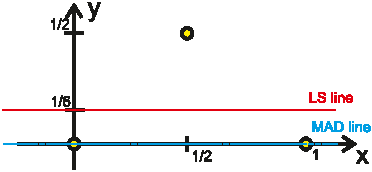
\includegraphics[scale=2.0]{obrazky/obrazek_1_F.pdf}
\end{center}

\end{example}


\begin{remark}
I když $ s^{2}_{n} $ je nestranný odhad $ \sigma^{2} $, $ s_{n} $ je vychýlený odhad $ \sigma $!
Je to obecná vlastnost odhadů (nestranných) rozptylů, neboť $ s^{2} $ nestranný odhad $ \sigma^{2} \, \Rightarrow \mathbb{E}[s] \leq \sigma $ 
\end{remark}

Uvažujme náhodnou veličinu $ X $  pro kterou platí, že $ \textbf{Var} [ X ] < + \infty $
\begin{equation*}
\begin{aligned}
 \mathbb{E}[X^{2}] = \textbf{Var} [ X ] +  \mathbb{E}[X]^{2} \quad \text{dosazením} \quad X = s \quad \text{dostaneme} \\
  \mathbb{E}[s^{2}] = \textbf{Var} [ s ] +  \mathbb{E}[s]^{2}
 \end{aligned} 
\end{equation*}
\begin{equation}
\mathbb{E}[s]^{2} \leq \sigma^{2} \quad \mathbb{E}[s] \leq \sigma
\end{equation}
a rovnost nastává pokud $ \textbf{Var} [ s ] = 0 $.

Například pro normální chyby je $ s_{n}^{2} \, \propto \, \chi^{2} \, \Rightarrow \, \mathbb{E} [s_{n}] < \sigma $

\begin{remark}
	předpokládali jsme, že hdnoty $ x_{i} $ jsou dány přesně, což nemusí být vždy pravda. Často obě veličiny $ (x,y) $ jsou měřeny nepřesně. EIV models "error in variable" v těchto modelech jsou často preferovány jiné odhady než LSE. Populární metoda: total least squares (ortogonal least squares). Zde minimalizujeme $ \sum_{i=1}^{n} d_{i}^{2} $, kde $ d_{i} $ je minimální vzdálenost bodu a přímky (kolmice na přímku protínající bod). To znamená, že neupřednostňujeme veličinu $ x $, ale přistupujeme k $ x $ a $ y $ rovnoměrně.
\end{remark}
\begin{center}
    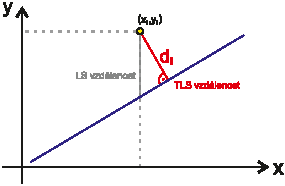
\includegraphics[scale=2.0]{obrazky/obrazek_2_F.pdf}
\end{center}

\begin{remark}
v literatuře se někdy $ x $ uvažují jako realizace náhodné veličiny ( ne vždy se $ x $ nastavuje předem, nebo je jasně dané (třeba pohlaví -- ???? (8 strana)) 
\end{remark}
Model má potom tvar
\begin{equation}
 \mathbb{E}[ Y_{i} \vert X_{i} ] = \beta_{0} + \beta_{1} \quad  \textbf{Var} [ Y_{i} \vert X_{i} ] = \sigma^{2}
\end{equation}
pro většinu výsledků prezentovaných v této přednášce ale není podstatné, zde je $ x $ chápáno jako pevné nebo náhodné.
Důkazy většinou fungují s podmíněnými výrazy $ ( \mathbb{E}, \textbf{Var} , \dots )  $ při dané hodnotě $ x $ místo nepodmíněných.
Nicméně větší pozornost je třeba u odvození asymptotických rozdělení odhadů.

\subsection{Vlastnosti odhadů}
Vlastnosti odhadů $ \widehat{\beta}_{0} , \widehat{\beta}_{1} ,  s_{n}^{2} $.
\begin{theorem}
   Nechť $ \widehat{\beta}_{0} , \widehat{\beta}_{1} $ jsou $ \LSE $ odhady parametrů $ \beta_{0}, \beta_{1} $ v lineárním modelu 
   \begin{equation}
   		Y_{i} = \beta_{0} + \beta_{1} x_{i} + e_{i} \quad i = 1 , \dots , n ,
   \end{equation}
   kde $ e_{i} $ jsou nezávislé náhodné veličiny (postačí i nekorelovanost) se stejným rozptylem $ \sigma^{2} $. Potom platí:
   \begin{enumerate}
  \item $ \E [ \widehat{\beta}_{0} ] = \beta_{0} \quad , \quad \E [ \widehat{\beta}_{1} ] = \beta_{1} $ , (nestranné odhady)
  \item $  \D [ \widehat{\beta}_{0} ] = \frac{\sigma^{2}}{S_{xx}}  \quad $ , kde $ \quad S_{xx} = \sumin (x_{i} - \oxnn )^{2} $
  \item $ \D [ \widehat{\beta}_{0} ] = \sigma^{2} \left( \frac{1}{n} + \frac{\oxnn ^{2}}{S_{xx}} \right) $
  \item Pokud navíc platí, že $ e_{i} \sim \NN ( 0 , \sigma^{2} ) \quad i = 1 , \dots , n \quad $ potom $ \quad \widehat{\beta}_{j} \sim \NN ( \beta_{j} , \D [ \widehat{\beta}_{j} ] ) \quad j = 0 , 1  $ 
\end{enumerate}
\end{theorem}
\begin{proofname}

   \begin{enumerate}
  \item upravíme $ \widehat{\beta}_{1} $
  		\begin{equation*}
  		\begin{aligned}
  		    \widehat{\beta}_{1} = \dfrac{\sum_{i=1}^{n} y_{i} x_{i} - n \overline{x}_{n} \overline{y}_{n}}{\sum_{i=1}^{n} x_{i}^{2} - n \overline{x}_{n}^{2}} = \frac{\sumin (x_i - \oxnn )(y_i - \oynn )}{\sumin (x_i - \oxnn )^{2}} = \\
  		    = \frac{1}{S_{xx}} \left( \sumin (x_i - \oxnn ) y_i - \oynn \sumin (x_i - \oxnn )  \right) =  \frac{1}{S_{xx}} \sumin (x_i - \oxnn ) y_i 
  		    \end{aligned}
  		\end{equation*}
  		potom má střední hodnota $ \widehat{\beta}_{1} $ tvar
  		\begin{equation*}
  		\begin{aligned}
  		    \E [ \widehat{\beta}_{1} ] = \E \left[ \frac{1}{S_{xx}} \sumin (x_i - \oxnn ) Y_i \right] = \frac{1}{S_{xx}} \sumin (x_i - \oxnn ) \E [ Y_i ] 
  		    = \frac{1}{S_{xx}} \sumin (x_i - \oxnn ) ( \beta_{0} + \beta_{1} x_i ) = \\ = \frac{\beta_{0}}{S_{xx}} \sumin (x_i - \oxnn ) + \frac{\beta_{1}}{S_{xx}} \sumin (x_i - \oxnn ) x_i = 0 + \frac{\beta_{1}}{S_{xx}} S_{xx} = \beta_{1}
  		    \end{aligned}
  		\end{equation*}
  		a střední hodnota pro $ \widehat{\beta}_{0} $ má tvar 
  		\begin{equation*}
  		\begin{aligned}
  		    \E [ \widehat{\beta}_{0} ] = \E [ \oyn - \widehat{\beta}_{1} \oxn ] = \E [ \oyn ] - \oxnn \E [ \widehat{\beta}_{1} ] = \dfrac{1}{n} \sumin \E [ Y_i ] - \oxnn \beta_1 = \beta_0 + \frac{\beta_1}{n} \sumin x_i - \oxnn \beta_1 = \beta_0
  		    \end{aligned}
  		\end{equation*}
  \item \begin{equation*}
  			\D [ \widehat{\beta}_{1} ] = \D \left[ \frac{1}{S_{xx}} \sumin (x_i - \oxnn ) Y_i \right] = \frac{1}{S_{xx} ^{2}} \sumin (x_i - \oxnn )^{2} \D [ Y_i ] = \frac{\sigma^{2} S_{xx}}{S_{xx}^{2}} = \frac{\sigma^{2}}{S_{xx}}
  		\end{equation*}
  \item  \begin{equation*}
  \begin{aligned}
  			\D [ \widehat{\beta}_{0} ] = \D [ \oyn - \widehat{\beta}_{1} \oxnn ] = \d [ \oyn ] + \oxnn ^{2} \D [ \widehat{\beta}_{1} ] - 2 \oxnn \text{cov}(\oyn , \widehat{\beta}_{1} ) = \\
  	= \frac{\sigma^{2}}{n} + \frac{\oxnn ^{2} \sigma^{2} }{S_{xx}} - 2 \oxnn \text{cov}( \oyn ,  \widehat{\beta}_{1} ) \\
\text{cov}( \oyn ,  \widehat{\beta}_{1} ) = \text{cov} \left( \oyn , \frac{1}{S_{xx}} \sumin ( x_i - \oxnn ) Y_i \right) = \frac{1}{S_{xx}} \sumin ( x_i - \oxnn ) \, \text{cov} ( \oyn , Y_i )  \\
\text{cov} ( \oyn , Y_i ) = \text{cov} ( \frac{1}{n} \sumjn Y_j , Y_i ) =  \frac{1}{n} \sumjn \text{cov} ( Y_j , Y_i ) = \frac{1}{n} \text{cov} ( Y_i , Y_i ) =  	\frac{1}{n} \D Y_i =  \frac{\sigma^{2}}{n}	\\
\Rightarrow  \text{cov}( \oyn ,  \widehat{\beta}_{1} ) = 0 = \frac{\sigma^{2}}{n S_{xx}} \sumin ( x_i - \oxnn )	
  			\end{aligned}
  		\end{equation*}
\end{enumerate}
\end{proofname}




\end{document}


